The focus in this section is on interactions occurring between multiple FAK molecules, which are obtained from setup 4. At this point the reader shall be reminded, that the used protein structure lacks the FAT domain, which is in full length FAK connected to the kinase via a linker region. This might make an important difference for clustering processes.
\subsection{Dimerization of FAK}
\label{mult:dimers}
First interactions between two FAK molecules are investigated. For this purpose the dataset was filtered for interactions, in which both partners have exactly one neighbour. As one can see in \autoref{linktoplot} FERM-kinase occurs the most followed by FERM-FERM dimers. Because FERM-FERM dimers have been experimentally investigated by \textcite{fakdimers} a short comparison between the obtained results and the experimental findings is given. For this purpose the dimer with the longest lasting time was chosen from the trajectories.\\ 
\\
The contact map of the interaction surface is shown in \autoref{interactioncontacts}. From this the importance of residue \acid{W}{266} can be confirmed (orange region). Beside this also the residues \acid{Y}{282} to \acid{K}{286} (green region), \acid{T}{291} to \acid{A}{394} (red region) and \acid{G}{322} to \acid{L}{327} (violet region) are important actors at the interaction surface since they interact with \acid{W}{266} and among each other. However, the RMSF value of these contacts is larger than for the contacts involving \acid{W}{266}.\\
At this point it has to be said that other FERM-FERM dimers in the simulation show also contacts between F1 and F3. Since they are not visible in other samples (e.g. the chosen one), they are not presented here.\\ 
FERM-FERM dimerization affects the FERM kinase interface of the involved proteins. In comparison to FAK-MEM almost all distances of the interacting residues gets closer for both protein instances (about $0.2\,\si{\nano\metre}$). A reason for this could be that the connection of the FERM domains require an uplift of F3 since the interaction interface points towards the membrane in FAK-MEM. Because the FERM domain is anchored on the membrane via the basic patch, this would push the kinase partly into the membrane. Therefore a force is acting on the kinase, which could be the reason of the closure. % TODO: cite Daniel?
\subsection{FAK clusters}
\label{mult:oligs}
The characterisation of the emerged FAK clusters is very difficult as they differ a lot in size and shape. The largest cluster observed in setup 4 had a size of 21 proteins, while there are other proteins, which did not join any cluster at all. Present shapes of the clusters include long chains as well as ring like conformations or just an agglomeration (see \autoref{tobeadded}). \\
\\
First of all the mean number of neighbours is considered. \autoref{mult:nng_vs_t} shows a fast rise in the number of neighbours in the beginning and a flattening after $6\,\si{\nano\second}$. The average of the five copies is at the end of the simulation $1.86$. This indicates a tendency to chains of FAK.\\
In \autoref{mult:inttype_vs_t} the time evolution of the average number of encounters of the different interaction types is determined. It shows, that FERM-kinase interactions (type 3) occur the most, while the others occur equally often. Only type 6 and type 7 (interactions, in which all four domains are involved) occur much less than the others.\\
From these observations one could draw the conclusion, that the preferred arrangement of FAK molecules is a chain, in which the FERM domain interacts with the kinase of the next molecule (FK-Chain). A second possibility would be a chain in which the FERM domain interacts with the FERM domain of the next molecule, while the kinase interacts with the kinase of the previous molecule (FFKK-Chain). It has to be noted that in the latter case the total number of interactions splits on two types while in the first case only one type occurs.
%
%
%
\begin{figure}
	\subcaptionbox{Mean number of neighbours against the time\label{mult:nng_vs_t}. Filled area is observed minimum and maximum.}[0.49\textwidth]{
		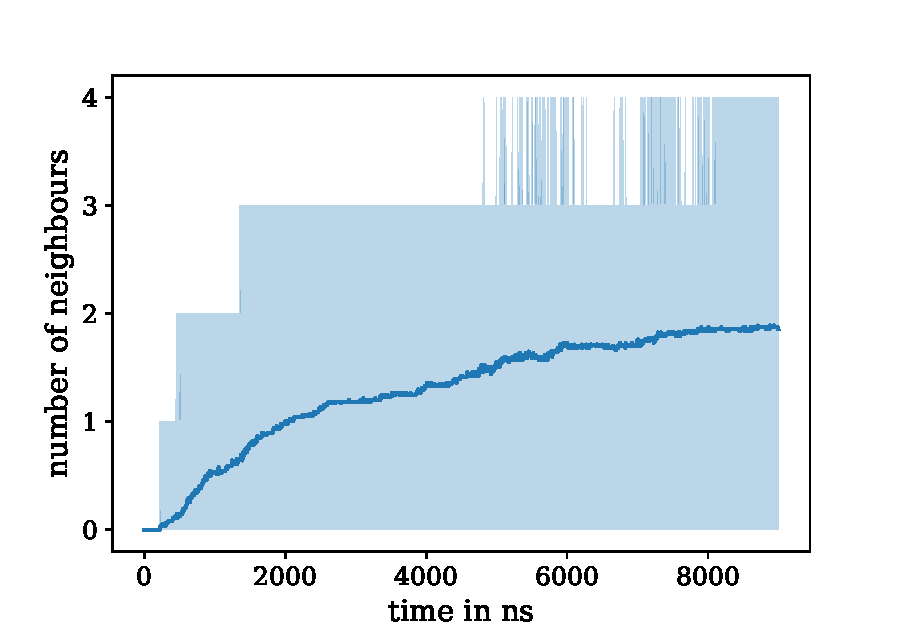
\includegraphics[height=5cm]{figures/results/averagenumber}
	}\hfill%
	\subcaptionbox{Mean number of interactions against the time\label{mult:inttype_vs_t}. Filled area is observed minimum and maximum.}[0.49\textwidth]{
		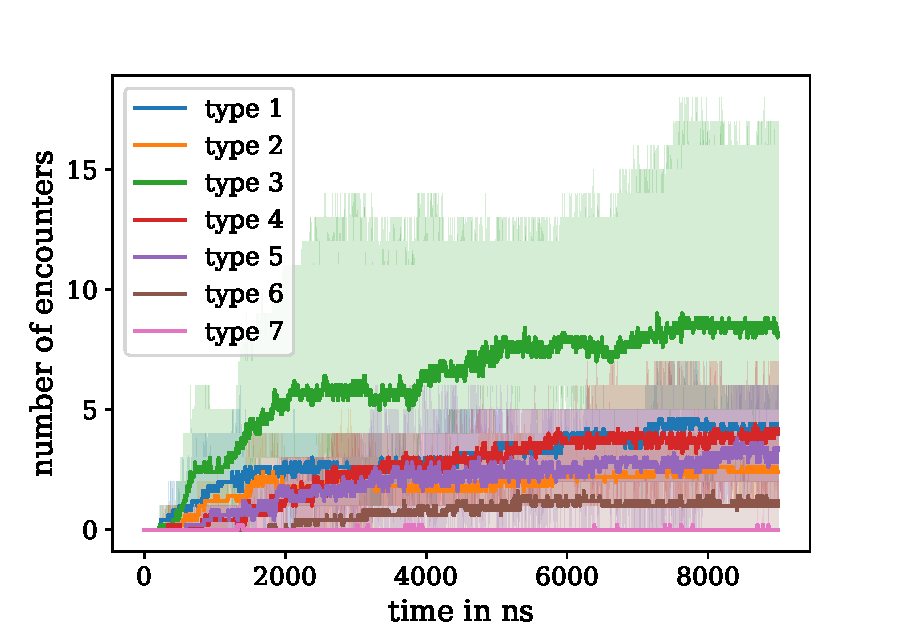
\includegraphics[height=5cm]{figures/results/multiple_typevstime}
	}%
	\phantomsubcaption
\end{figure}
%
%
%
\subsection{Activation due to clustering}
At last, the impacts of clustering on FAK activation are addressed. Activation means here the dissociation of the FERM domain from the kinase, therefore the obtained trajectories are analysed with respect to the contact area (CA) of the FERM-kinase interface.\\
Unfortunately in no FAK molecule a full dissociation took place at any time. Because only a small number of FAK molecules were in the system and because the clustering process is not finished at the end of the simulations, this does not mean, that activation due to clustering would not be possible at all. In the hope of seeing trends regarding to activation a more detailed analysation of the CA for the different proteins was performed.\\
\\
CA seems to be independent of the number of neighbours (\autoref{bild}), the interaction type and the clustersize. Therefore the data was filtered more.\\
Motivated from \autoref{mult:dimers} and \autoref{mult:oligs}, only FAK molecules inside chains are taken into account. A FAK molecule can be seen as a chain member, if it has exactly two neighbours and if these neighbours are not neighbours of one another. For FK chains only type 3 interactions were allowed, for FFKK chains both, type 1 and type 2. The resulting distribution of CA as well as the COM distances $d_\text{F1-N}$ and $d_\text{F2-C}$ can be found in \autoref{mult:fk_ca} for FK chains and in \autoref{mult:ff_ca} for FFKK chains.\\
\autoref{mult:fk_ca} indicates that an arrangement of FAK molecules to FK chains does not influence the mean value of CA. The distribution gets slightly sharper compared to FAK-MEM, which could imply a stabilisation of the interface. The Q-Q plot in \autoref{figure} indicates that not even the distributions of $d_\text{F1-N}$ and $d_\text{F2-C}$ differs from those obtained in FAK-MEM.\\
Also an arrangement to FFKK chains affects the value of CA hardly (\autoref{figure}). The distribution gets slightly sharper and shifted to smaller values by $0.6\,\si{\nano\metre}$. In contrast the Q-Q plot of $d_\text{F1-N}$ in \autoref{figure} indicates a trend to larger values than obtained for FAK-MEM.\\
\\
The filtering leads of course to a smaller sampling of the distributions of $d_\text{F1-N}$, $d_\text{F2-C}$ and CA . E.g. for FFKK chains only 10 different FAK instances spanning a simulation time of $21.7\,\si{\micro\second}$ in total were taken into account. However the obtained changes are visible in almost all of the 10 instances.
%
%
%
\begin{figure}
	\centering
	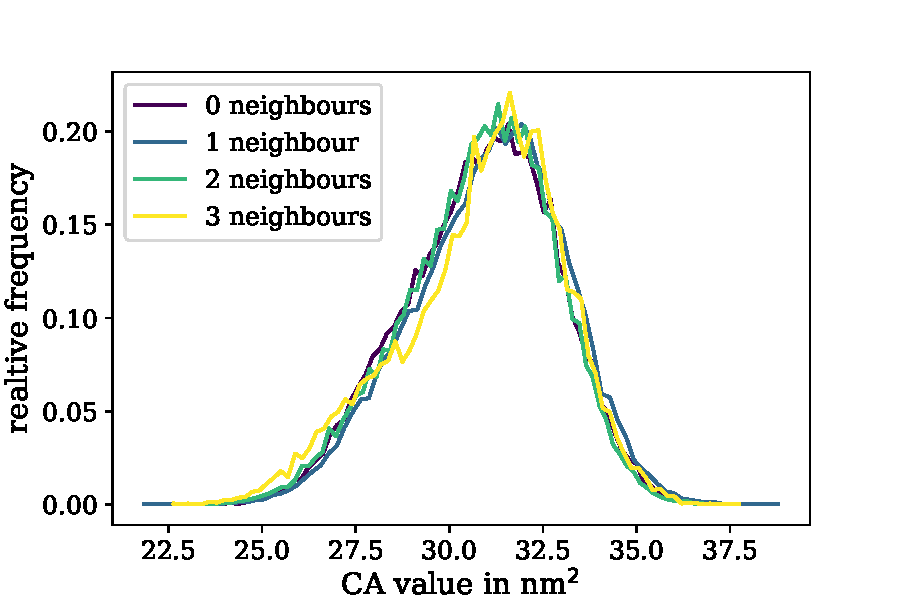
\includegraphics[height=6cm]{figures/results/nng_ca}
	\captionof{figure}{CA for different number of neighbours}
	\label{mult:nng_ca}
\end{figure}
%
%
%
%
%
%
\begin{figure}
	\centering
	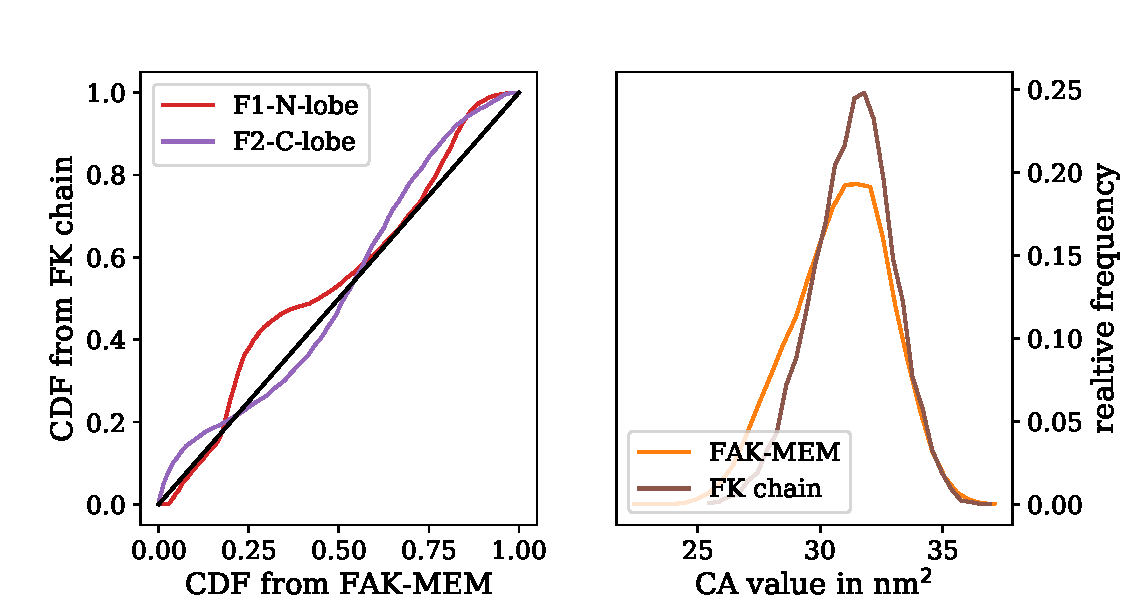
\includegraphics[height=6cm]{figures/results/fk_ca}
	\captionof{figure}{Analysis of the FERM-kinase interface in FK-Chains. The blue line was obtained from FAK-MEM.}
	\label{mult:fk_ca}
\end{figure}
%
%
%
%
%
%
%
\begin{figure}
	\centering
	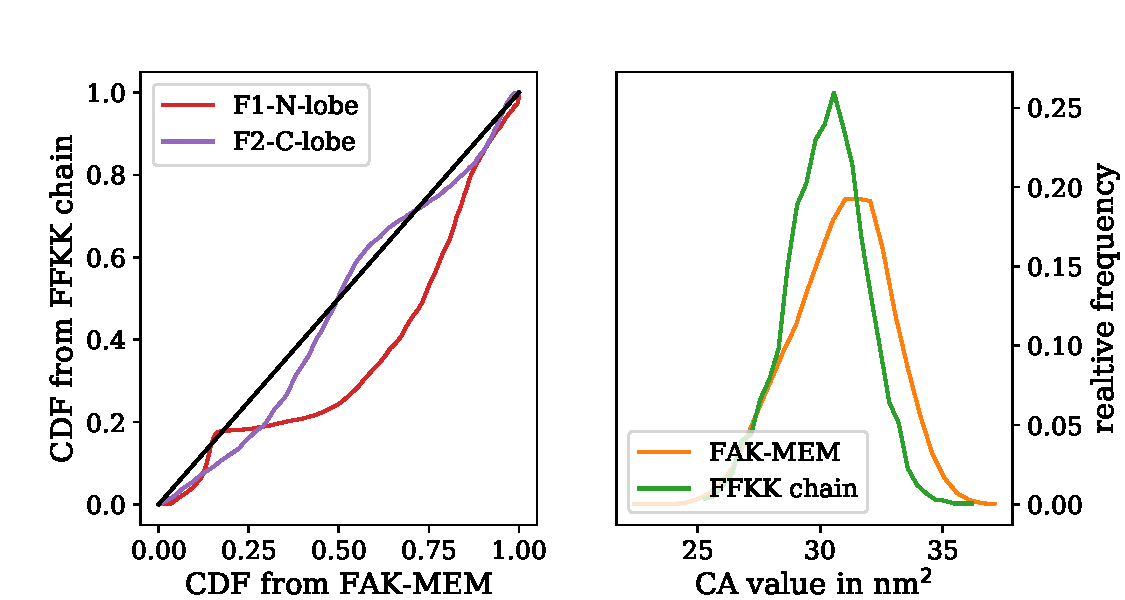
\includegraphics[height=6cm]{figures/results/ff_ca}
	\captionof{figure}{Analysis of the FERM-kinase interface in FFKK-Chains. The blue line was obtained from FAK-MEM.}
	\label{mult:ff_ca}
\end{figure}
%
%
%
%

